\documentclass[letterpaper]{article} % DO NOT CHANGE THIS
\usepackage{aaai2027}  % DO NOT CHANGE THIS
% The serif, sans-serif, and monospaced fonts are loaded automatically by
% aaai2027.sty (newtxtext, helvet, courier). DO NOT add font packages.
\usepackage[hyphens]{url}  % DO NOT CHANGE THIS
\usepackage{graphicx} % DO NOT CHANGE THIS
\urlstyle{rm} % DO NOT CHANGE THIS
\def\UrlFont{\rm}  % DO NOT CHANGE THIS
\usepackage{natbib}  % DO NOT CHANGE THIS AND DO NOT ADD ANY OPTIONS TO IT
\usepackage{caption} % DO NOT CHANGE THIS AND DO NOT ADD ANY OPTIONS TO IT
\frenchspacing  % DO NOT CHANGE THIS
\usepackage{booktabs}

% Keep the \pdfinfo as shown here. There's no need
% for you to add the /Title and /Author tags.
\pdfinfo{
/TemplateVersion (2027.1)
}

\setcounter{secnumdepth}{0}

% Pack the trailing full-width figures instead of leaving near-empty
% float pages (7 wide figures against ~4.5 pages of text).
\renewcommand{\dbltopfraction}{0.95}
\renewcommand{\dblfloatpagefraction}{0.9}
\setcounter{dbltopnumber}{3}

% The course guidelines advise removing the AAAI copyright footnote.
\nocopyright

\graphicspath{{../final_results/course_paper/figures/}}

\title{Graph Card Control: Evaluating Search Agents in a Stochastic Abstract Strategy Game}
\author{
    Omri Avital (208693341)\quad
    Itai Reder (318850781)
}
\affiliations{
    237-2-5513 Search Methods in Artificial Intelligence
}

\begin{document}

\maketitle

\begin{abstract}
We introduce Graph Card Control, a configurable two-player, stochastic, perfect-information game for controlled comparison of bounded search implementations and transparent baselines. The only random event is replacement of a selected card in a three-card public market. We evaluate random, greedy, rule-based, Monte Carlo tree search (MCTS), and depth-2/depth-3 expectimax agents across three board geometries, three stopping rules, player order, and independently varied deck composition. The corrected suite contains 1,116 replay-validated games and prevents agents from conditioning on hidden deck order. Rule achieved the highest aggregate win-points rate (66.0\%) at 4.8 ms per decision. Among search agents, Expectimax d3 reached 63.6\% at 956.3 ms. Depth-3 expectimax cost 8.6 times depth 2 and obtained 52.8\% in their direct matches. Board geometry, stopping rule, deck composition, and player order all changed outcomes. The results characterize these fixed-budget implementations; they are not universal algorithm rankings.
\end{abstract}

\section{Introduction and Literature Review}

Game playing provides a controlled setting in which states, actions, stochastic transitions, and utility can be specified exactly. This project asks a narrower empirical question: when an unfamiliar game combines adversarial choice with a public stochastic card refill, how do bounded search agents compare with transparent baselines under changes to geometry, stopping rule, deck composition, and move order? The course explicitly identifies a custom strategy game with search-based and threshold agents as a suitable research direction.

Graph Card Control is a stochastic, perfect-information game. Exact lookahead therefore requires decision nodes for both players and expectation over replacement-card outcomes. Ballard's *-minimax analysis showed how bounds can prune trees containing chance nodes \citep{ballard1983}, while Monte Carlo *-minimax later combined sparse sampling with stochastic adversarial search \citep{lanctot2013}. These works motivate expectimax as the structurally appropriate exact model and also predict its computational difficulty when both action and chance branching are present.

MCTS offers an alternative allocation of computation. \citet{coulom2006} integrated Monte Carlo evaluation with selective tree growth, and \citet{kocsis2006} introduced UCT, establishing consistency and finite-sample error bounds for Monte Carlo planning. Sparse sampling can avoid enumerating every stochastic successor \citep{kearns1999}. Our corrected MCTS samples replacement cards from the public composition on every traversal, aggregates outcomes on stochastic action edges, and treats the opponent as a minimizing player. Expectimax instead enumerates the complete known refill distribution after selecting its bounded action beam.

The broader MCTS literature separates selection, expansion, simulation, and backup, with playing strength depending on choices in every phase \citep{browne2012}. This matters for interpretation: our comparison tests one explicit budget and rollout design, while expectimax spends computation on exhaustive chance backup inside a depth limit. A result for either implementation is therefore evidence about a cost-allocation choice, not about all members of the algorithm family.

Deeper search is not automatically better when leaf evaluation is approximate. \citet{pearl1983} demonstrated that repeated minimax backup can amplify evaluation noise and, in pathological cases, degrade decisions with depth. The choice-function framework likewise formalizes when pruning the considered action set can preserve policy improvement \citep{issakkimuthu2020}. These results are directly relevant to our top-2 expectimax cap and to interpreting the observed depth/runtime trade-off rather than treating depth as an unconditional quality scale.

We organize the evaluation around five questions. Which agent is strongest across the chosen boards and stopping rules? How much decision time does that performance require? Does moving first change the comparison? Does independently changing the deck alter the ranking? Finally, do deeper expectimax and the net-launcher mechanic produce evidence of qualitatively different play? These are descriptive questions about the implemented system; they are not claims of universal algorithm superiority.

General game playing emphasizes evaluating agents on games not engineered around a single solver \citep{genesereth2005}. Our contribution is accordingly methodological rather than algorithmic: (i) an executable stochastic game with configurable geometry, objectives, decks, and stopping rules; (ii) a reproducible matched-order experiment system; and (iii) an empirical comparison that includes computational cost and behavior, not only win rate.

\begin{figure*}[t]
\centering
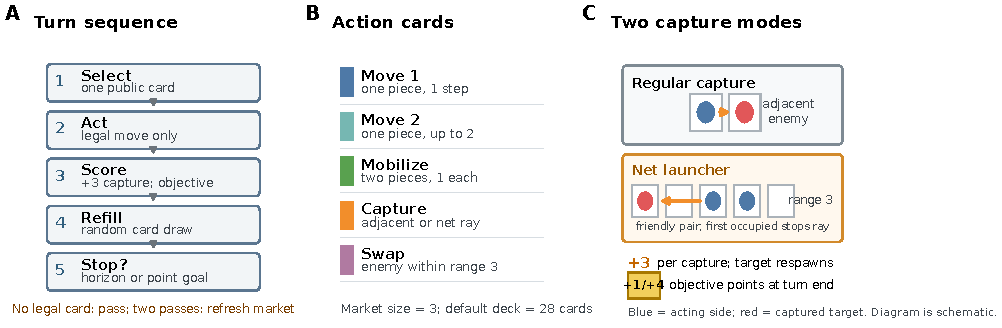
\includegraphics[width=\textwidth]{01_game_mechanics}
\caption{\textbf{Turn structure and capture modes.} \textbf{(A)} The player selects a public card, acts, scores, refills the market randomly, and tests the stopping rule. With no legal card the player passes; two passes refresh the market. \textbf{(B)} The five card types and their ranges. Mobilize moves two pieces when possible and otherwise one. \textbf{(C)} A regular (melee) capture targets an orthogonally adjacent enemy. A net launcher uses an adjacent friendly pair and the first occupied cell on an outward range-3 ray. Both score three points and respawn the target; objective cells score at turn end. Blue is the acting side and red the target; diagrams are schematic.}
\label{fig:mechanics}
\end{figure*}

\section{Methodology}

\subsection{Game model}

Players alternate turns on an orthogonal grid and control three pieces each. The current player selects one legal action from a public three-card market. Movement cards reposition pieces; Capture scores three points through an adjacent attack or net launcher; Swap exchanges a friendly and enemy piece within Manhattan distance three. Captured pieces respawn, preventing elimination. Objective cells score at the end of every occupying turn. After a played card is discarded, its market slot is refilled by a draw from the known remaining composition. Thus the state is fully observable while the next refill is stochastic (Figure 1).

A pass occurs only when all visible cards are unusable. Preliminary experiments identified repeated passes as an absorbing market failure, so every final condition refreshes all three market cards after two consecutive passes. Any legal move resets the counter. This rule change is fixed across the final suite and is not itself an experimental factor.

\subsection{Implementation}

The Python 3.10+ rules engine represents a state as an immutable record and applies actions through a shared transition function. Random-number-generator state is carried inside the game state, making a game deterministic once its seed is fixed. Legal-action generation and state transitions are shared by human, baseline, and search agents, preventing agent-specific rule implementations. Runtime dependencies and analysis libraries are declared in the repository requirements file.

Replacement draws can be forced during search and replay. Agents receive the executable state, which retains a shuffled deck for deterministic match execution, but corrected successor evaluation never consults that hidden ordering. Greedy and rule-based evaluation use a deterministic most-probable public refill solely for action ordering. Expectimax backs up the exact probability-weighted value of every remaining card type; its top-2 beam is ordered in the appropriate maximizing or minimizing direction. MCTS resamples the public draw distribution with an agent-local random generator on every action-edge traversal and alternates root-player maximization with opponent minimization (100 simulations, rollout depth 10, exploration constant 1.4). Reversing the hidden deck while holding all public fields fixed changed zero tested choices for greedy, rule, expectimax depth 2, and MCTS.

\begin{figure*}[t]
\centering
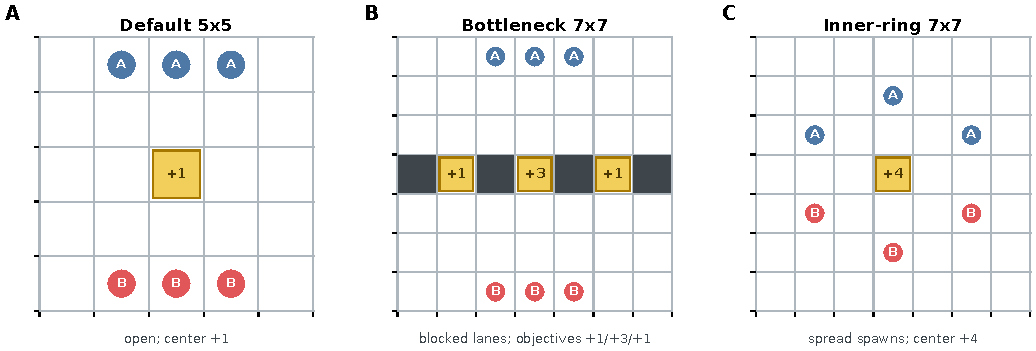
\includegraphics[width=\textwidth]{02_experimental_boards}
\caption{\textbf{Three board geometries define the spatial experimental factor.} \textbf{(A)} Default open 5x5 board. \textbf{(B)} Bottleneck 7x7 board with blocked central lanes. \textbf{(C)} Inner-ring 7x7 board with more widely separated spawns and a four-point center. Blue and red circles mark the initial cells of players A and B; yellow cells are end-of-turn objectives labeled by points; dark cells are blocked. Coordinates and piece identities are omitted because the JSON board definitions are the authoritative executable specification.}
\label{fig:boards}
\end{figure*}

\subsection{Boards, decks, and stopping rules}

The main factorial varies three symmetric boards (Figure 2) and three stopping rules: a fixed 25 turns per player, first to 10 points, and first to 40 points. Goal games retain a 50-turn-per-player safety cap. Goal 10 emphasizes openings, whereas goal 40 permits sustained positional control. The inner-ring center awards four points, deliberately making center occupation more valuable than a three-point capture.

Deck composition is tested independently on the default board at the fixed horizon. The 28-card control deck contains 8 Move 1, 6 Move 2, 5 Mobilize, 5 Capture, and 4 Swap cards. Movement-, capture-, and swap-heavy variants alter these counts without changing card behavior. This reduced design avoids an uninterpretable full cross-product while preserving a common control.

\subsection{Agents}

Random samples uniformly from legal actions. Greedy selects the immediate public-information successor with the highest shared heuristic. Rule prioritizes captures and objectives, then uses that heuristic for tie-breaking. Expectimax alternates maximizing and minimizing decision nodes and expands exact replacement-card probabilities at depth 2 or 3; its top-2 beam keeps the best root-player actions at maximizing nodes and the strongest replies at minimizing nodes. MCTS uses 100 simulations, rollout depth 10, sampled public chance outcomes, and adversarial selection. Deterministic minimax is excluded because it neither models chance nodes nor answers the stochastic-search question.

The shared evaluation is a weighted difference between the players: score (100), objective-cell control (10), distance to the nearest objective (2), capture threats (15), net-launcher potential (20), swap potential (8), piece safety (10), and legal-action mobility (1). The dominant score weight encodes the game objective; all weights are fixed across final conditions and stored in every mode configuration.

\subsection{Experimental design and metrics}

Each board/stopping-rule condition contains every ordered non-self pair among six agents and three matched game seeds (90 games). Mirrored orders reuse the seed, allowing direct first-versus-second comparison. Four independent deck conditions contribute 360 games, but the default fixed-horizon control is shared with the board study; the 12 unique main/deck modes therefore contain 1,080 games. A bounded goal-20 depth study adds 36 games across the three boards, for 1,116 total.

A win contributes one win point, a draw one half, and a loss zero. The engine measures each action-selection call with a monotonic high-resolution clock; runtime is total logged decision time divided by non-pass decisions. The corrected suite ran sequentially on an Intel Core i5-9600K under 64-bit Python 3.12.13 and Windows 10 (build 19045), so timing supports within-machine comparisons rather than portable benchmarks. Behavioral analysis reconstructs adjacent and net-launcher captures from per-turn logs. Percentages are descriptive: a direct main matchup has six games, and the same seeds recur across conditions. Each mode stores its complete configuration. All 1,116 logs replayed from forced draws matched the recorded final outcomes.

\subsection{Analysis plan}

The primary comparison asks which agents perform well across boards and stopping rules. Secondary analyses examine first-versus-second order, performance per unit decision time, isolated deck composition, direct expectimax-depth matchups, and adjacent versus net-launcher captures. The deck study is analyzed separately because it was deliberately not crossed with board geometry.

No null-hypothesis significance tests or confidence intervals are reported. Games within a matched seed and repeated conditions are not independent, while direct matchups contain only six games. The analysis therefore reports denominators, matched contrasts, and calibrated descriptive conclusions; confirmatory inference is left to a larger independent-seed experiment.

\begin{figure*}[t]
\centering
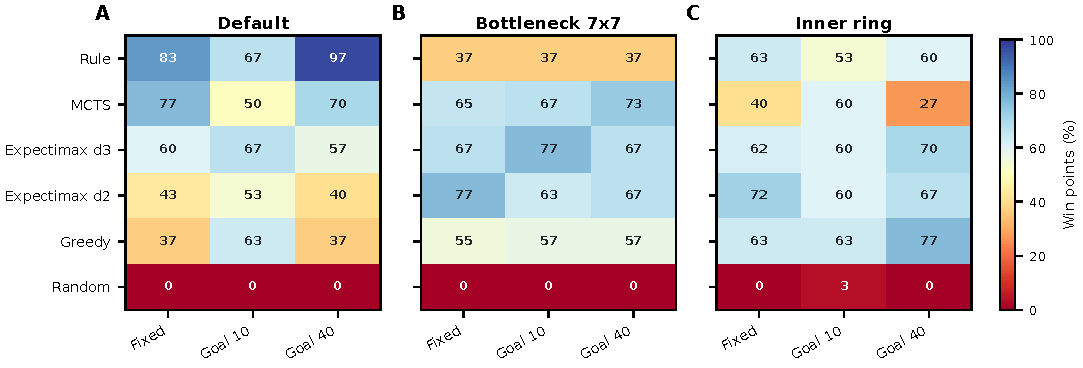
\includegraphics[width=\textwidth]{03_board_goal_performance}
\caption{\textbf{Agent rankings vary across board geometry and stopping rule.} \textbf{(A-C)} Win points for the six agents on the default, bottleneck, and inner-ring boards, respectively. Columns are a fixed 25-turn-per-player horizon and point goals of 10 or 40; the turn cap remains a safety bound in goal games. Each cell contains 30 agent-game observations: five opponents, both player orders, and three matched seeds. A win contributes 1, a draw 0.5, and a loss 0. Color and printed values both encode win points (\%); 50\% denotes parity across opponents. Conditions are separate tests, not pooled replicates.}
\label{fig:board_goal}
\end{figure*}

\section{Experimental Results}

\subsection{Overall performance}

Across the 12 unique main and deck conditions, the aggregate order was Rule (66.0\%), Expectimax d3 (63.6\%), MCTS (62.4\%), Expectimax d2 (56.8\%), Greedy (51.0\%), Random (0.3\%). Rule therefore provided the strongest observed performance-cost trade-off at its measured budget. This pooled ranking is descriptive rather than universal: board geometry and stopping rule changed the relative ordering (Figure 3).

\begin{table}[t]
\centering
\caption{Aggregate results across the 12 unique main/deck conditions.}
\label{tab:overall}
\small
\begin{tabular}{lrrrr}
\toprule
Agent & N & Win points & Margin & ms/decision \\
\midrule
Rule & 360 & 66.0\% & +10.31 & 4.76 \\
MCTS & 360 & 62.4\% & +6.36 & 166.94 \\
Expectimax d3 & 360 & 63.6\% & +8.37 & 956.34 \\
Expectimax d2 & 360 & 56.8\% & +6.77 & 110.88 \\
Greedy & 360 & 51.0\% & +5.30 & 9.42 \\
Random & 360 & 0.3\% & -37.11 & 0.00 \\
\bottomrule
\end{tabular}
\end{table}

\subsection{Board geometry and stopping rule}

The heatmaps show that no pooled percentage captures every condition. Goal-10 games were especially short on the four-point inner-ring board, where one or two successful center occupations can determine the result. Mean combined duration was 13.8, 15.5, and 6.7 turns for goal 10 on the default, bottleneck, and inner-ring boards, respectively, compared with 58.5, 35.0, and 22.4 turns for goal 40. Goal 10 is therefore an opening-focused stress test rather than a substitute for longer evaluation.

\subsection{Runtime and move order}

Performance did not increase monotonically with decision time (Figure 4A). Measured costs were 4.8 ms for rule, 9.4 ms for greedy, 110.9 ms for expectimax depth 2, 166.9 ms for MCTS, and 956.3 ms for expectimax depth 3. Depth 3 was 8.6 times slower than depth 2, while their aggregate win-points difference was +6.8 percentage points. Additional lookahead changed decisions, but its cost was not matched by a uniform direct advantage.

Move-order effects were smaller than the full spread between agents but remained visible (Figure 4B). The largest absolute first-minus-second contrast was +8.1 percentage points for MCTS; MCTS was +8.1, depth-3 expectimax \mbox{-0.6}, and rule +4.7. Because every pair is mirrored with the same seed, these contrasts control opponent identity and the seeded refill process more closely than an unmatched tournament.

\begin{figure*}[t]
\centering
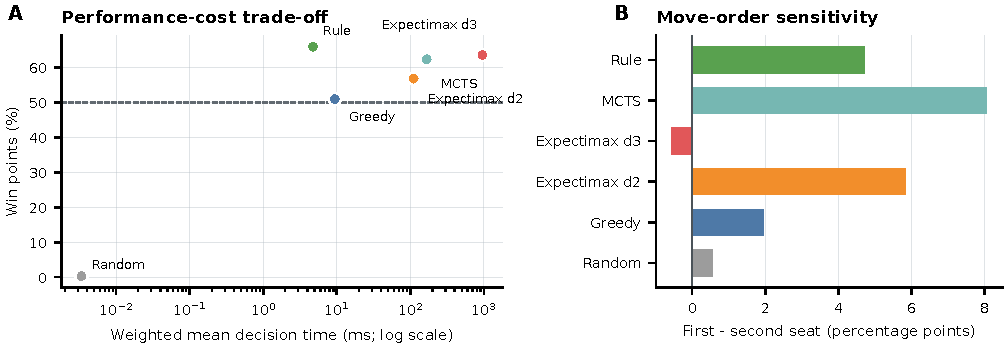
\includegraphics[width=\textwidth]{04_efficiency_and_order}
\caption{\textbf{Additional computation does not yield a monotonic performance gain.} \textbf{(A)} Aggregate win points versus weighted mean decision time across the 12 main and independent-deck conditions. Each agent has 360 agent-game observations; time is total recorded decision time divided by non-pass decisions and is shown on a logarithmic axis. The dashed line marks 50\% win points. \textbf{(B)} First-seat minus second-seat win-points rate for the same conditions (180 agent-game observations per seat and agent). Positive values favor moving first. Colors identify agents in both panels; labels provide a redundant non-color encoding.}
\label{fig:efficiency}
\end{figure*}

\subsection{Independent deck-composition test}

Changing card frequencies altered relative performance even though board, stopping rule, market refresh, and seed design were fixed (Figure 5). The leading agents were Default: Rule (83.3\%); Movement-heavy: Rule (83.3\%); Capture-heavy: Rule (81.7\%); Swap-heavy: Rule (93.3\%). Thus a ranking from one action distribution should not be generalized to the game family. Because deck and board were not crossed, this experiment estimates deck effects on the default board, not deck-by-geometry interactions.

\begin{figure*}[t]
\centering
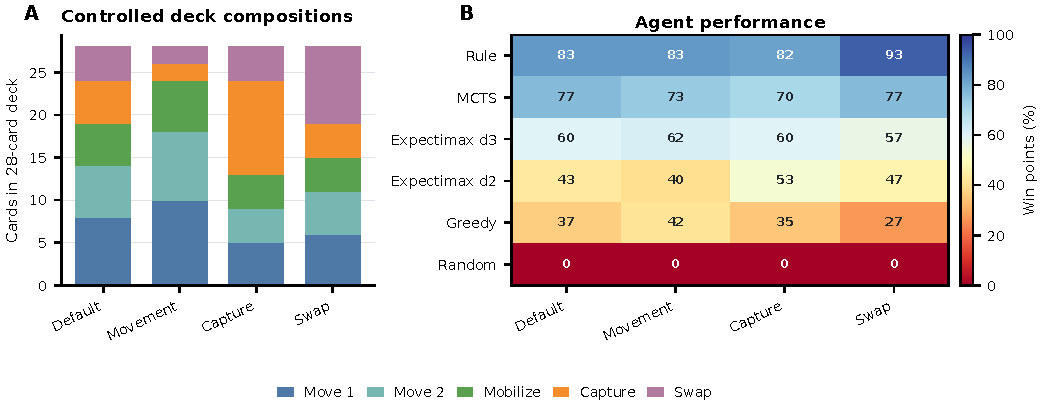
\includegraphics[width=\textwidth]{05_deck_composition}
\caption{\textbf{Independently changing deck composition shifts relative agent performance.} \textbf{(A)} Counts of the five action cards in each 28-card deck; stacked segments sum to 28. \textbf{(B)} Win points on the default board under the fixed 25-turn-per-player horizon. Each cell contains 30 agent-game observations across five opponents, both player orders, and three matched seeds. Color and printed values encode win points (\%). The default condition is the shared control; the three alternatives change only card counts while retaining the two-pass market refresh.}
\label{fig:decks}
\end{figure*}

\subsection{Expectimax depth}

Across nine direct board/stopping-rule cells, depth 3 obtained 52.8\% of win points against depth 2 over 54 agent-game observations (Figure 6A). The bounded study shows the computational reason for stopping at depth 4: runtime rises steeply on all boards (Figure 6B), while the corresponding performance estimates use only one seed and are unstable (Figure 6C). Depth 5 exceeded 120 seconds for one benchmark decision; depth 6 was therefore not run. The branching structure and approximate top-2 beam make this result plausible, but the experiment does not isolate a causal mechanism and does not establish search pathology.

\begin{figure*}[t]
\centering
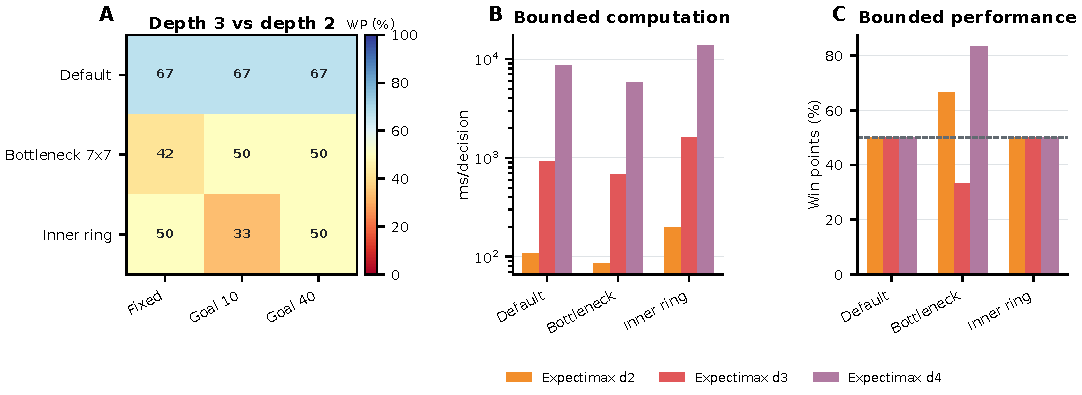
\includegraphics[width=\textwidth]{06_expectimax_depth}
\caption{\textbf{Deeper expectimax is substantially slower and is not uniformly stronger.} \textbf{(A)} Depth-3 win points in direct depth-3 versus depth-2 matches for all nine board/stopping-rule combinations. Each cell summarizes six games (three matched seeds in both player orders); 50\% denotes parity. \textbf{(B-C)} Weighted mean decision time and win points, respectively, in the bounded goal-20 feasibility study. Bars summarize six agent-game observations per board and depth; all variants use a top-2 action cap. Runtime uses a logarithmic axis and the dashed performance line marks 50\%. Depth 4 used one seed and is interpreted as a feasibility measurement; depth 5 exceeded 120 s for one benchmark decision and depth 6 was not run.}
\label{fig:depth}
\end{figure*}

\subsection{Dominant strategies and net-launcher use}

Rule is explicitly capture-first and objective-first, whereas greedy and expectimax optimize a broader multi-term heuristic that can trade immediate score for mobility, safety, or formation potential. In the main suite, Move 1 was every agent's most-used card (26.7-28.0\% of played actions), largely reflecting its 8/28 deck prevalence. Capture-card shares were also similar (19.0-20.3\%), while capture rates ranged from 3.32 to 3.82 per agent-game. These availability-conditioned summaries do not isolate a winning mechanism; that requires policy and heuristic-weight ablation. Complete action counts are available in the accompanying results archive (\texttt{tables/16\_action\_usage\_summary.csv}).

The net launcher accounted for 1,769 of 8,020 captures (22.1\%) across the complete suite. In the comparable 1,080-game main/deck suite, 1,729 of 7,863 captures were net launches (22.0\%; Figure 7). This frequency establishes that the mechanic affects play, but event counts alone do not establish that using it causes wins.

\begin{figure*}[t]
\centering
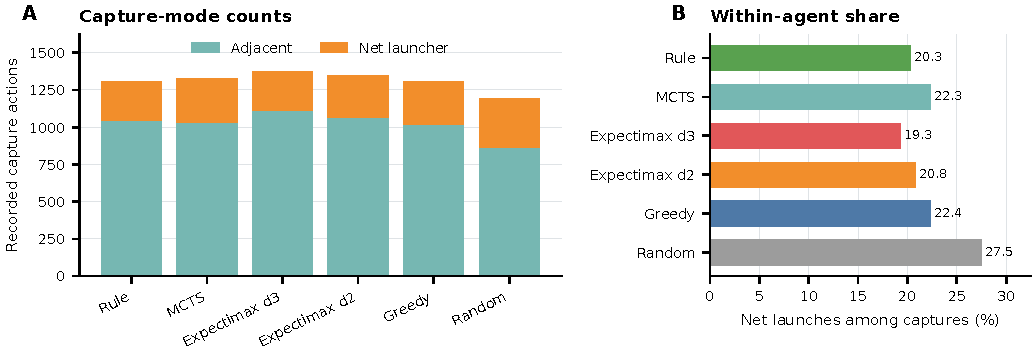
\includegraphics[width=\textwidth]{07_net_launcher}
\caption{\textbf{Net launches are a recurring but minority capture mode.} \textbf{(A)} Adjacent and net-launcher capture actions reconstructed from all per-turn logs in the 1,080-game main and deck suite (7,863 captures; 1,729 net launches). Counts are events, not games, and therefore reflect both opportunity and agent behavior. \textbf{(B)} Net launches as a percentage of each agent's captures, with exact percentages printed beside the bars. Expectimax depth 4 is excluded because it appears only in the smaller bounded feasibility study. Across the displayed agents, the net share ranges from 19.3\% (Expectimax d3) to 27.5\% (Random).}
\label{fig:net}
\end{figure*}

\section{Experimental Conclusions and Summary}

The project achieved its objective of constructing a reproducible stochastic game domain and comparing bounded search implementations with meaningful baselines. Under the tested settings, Rule produced the highest aggregate win-points rate, Expectimax d3 led the evaluated search agents, and depth-3 expectimax was substantially more expensive than depth 2 without a uniform direct advantage. Board geometry, score goal, deck composition, and player order all changed outcomes, so one pooled tournament ranking would obscure important structure.

The main limitations are statistical and budgetary. Direct depth matchups contain six games per condition, only three seeds support the main cells, seeds recur across conditions, and no confidence intervals are claimed. Decks were varied independently rather than factorially with boards. Expectimax retains a heuristic top-2 beam, depth 4 uses one seed, and MCTS samples rather than exhaustively expands chance outcomes. MCTS and expectimax were not matched by wall-clock budget, and the shared heuristic was not tuned on a separate training set. The corrected agents pass hidden-deck-order invariance tests, but the API still carries the execution deck, so architectural separation would be safer than relying on tested discipline. Future work should increase independent paired seeds, compare equal-time performance curves, ablate heuristic terms, and test *-minimax or progressive-widening variants where chance branching grows.

\subsection{Code and data availability}

Source code, board and deck definitions, experiment configurations, per-game results, move logs, analysis scripts, and figure-generation code are available at \url{github.com/Naharda/Grid_Control_Game}. The report figures are generated by \texttt{analysis/build\_course\_paper.py}; complete final-suite tables are indexed under \texttt{final\_results/}.

\bibliography{references}

\end{document}
